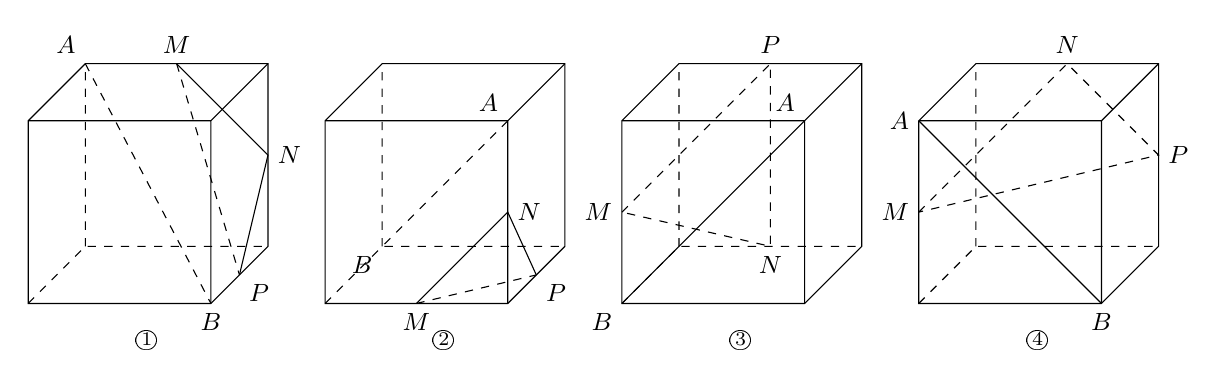
\begin{tikzpicture}[x=5.8mm,y=5.8mm,every node/.style={font=\small}]
  % Each cube uses the same perspective; its labelled vertices and midpoints differ.
  \begin{scope}[shift={(0,0)}]
    \coordinate (FBL) at (0,0); \coordinate (FBR) at (4,0);
    \coordinate (FTR) at (4,4); \coordinate (FTL) at (0,4);
    \coordinate (BBL) at (1.25,1.25); \coordinate (BBR) at (5.25,1.25);
    \coordinate (BTR) at (5.25,5.25); \coordinate (BTL) at (1.25,5.25);
    \coordinate (A) at (BTL); \coordinate (M) at (3.25,5.25);
    \coordinate (N) at (5.25,3.25); \coordinate (B) at (FBR);
    \coordinate (P) at (4.625,.625);

    \draw[dashed] (FBL)--(BBL)--(BBR) (BBL)--(BTL);
    \draw (FBL)--(FBR)--(BBR)--(BTR)--(BTL)--(FTL)--cycle;
    \draw (FTL)--(FTR)--(BTR) (FBR)--(FTR);
    \draw[dashed] (A)--(B) (M)--(P);
    \draw (M)--(N)--(P);

    \node[above left] at (A) {$A$};
    \node[above] at (M) {$M$};
    \node[right] at (N) {$N$};
    \node[below] at (B) {$B$};
    \node[below right] at (P) {$P$};
    \node[below=7pt] at (2.6,0) {\scriptsize\textcircled{1}};
  \end{scope}

  \begin{scope}[shift={(6.5,0)}]
    \coordinate (FBL) at (0,0); \coordinate (FBR) at (4,0);
    \coordinate (FTR) at (4,4); \coordinate (FTL) at (0,4);
    \coordinate (BBL) at (1.25,1.25); \coordinate (BBR) at (5.25,1.25);
    \coordinate (BTR) at (5.25,5.25); \coordinate (BTL) at (1.25,5.25);
    \coordinate (B) at (BBL); \coordinate (A) at (FTR);
    \coordinate (M) at (2,0);
    \coordinate (N) at (4,2); \coordinate (P) at (4.625,.625);

    \draw[dashed] (FBL)--(BBL)--(BBR) (BBL)--(BTL);
    \draw (FBL)--(FBR)--(BBR)--(BTR)--(BTL)--(FTL)--cycle;
    \draw (FTL)--(FTR)--(BTR) (FBR)--(FTR);
    \draw[dashed] (A)--(B) (M)--(P);
    \draw (M)--(N)--(P);

    \node[below left] at (B) {$B$};
    \node[above left] at (A) {$A$};
    \node[below] at (M) {$M$};
    \node[right] at (N) {$N$};
    \node[below right] at (P) {$P$};
    \node[below=7pt] at (2.6,0) {\scriptsize\textcircled{2}};
  \end{scope}

  \begin{scope}[shift={(13,0)}]
    \coordinate (FBL) at (0,0); \coordinate (FBR) at (4,0);
    \coordinate (FTR) at (4,4); \coordinate (FTL) at (0,4);
    \coordinate (BBL) at (1.25,1.25); \coordinate (BBR) at (5.25,1.25);
    \coordinate (BTR) at (5.25,5.25); \coordinate (BTL) at (1.25,5.25);
    \coordinate (B) at (FBL); \coordinate (A) at (FTR);
    \coordinate (M) at (0,2);
    \coordinate (N) at (3.25,1.25); \coordinate (P) at (3.25,5.25);

    \draw[dashed] (FBL)--(BBL)--(BBR) (BBL)--(BTL);
    \draw (FBL)--(FBR)--(BBR)--(BTR)--(BTL)--(FTL)--cycle;
    \draw (FTL)--(FTR)--(BTR) (FBR)--(FTR);
    \draw (A)--(B);
    \draw[dashed] (M)--(P)--(N)--cycle;

    \node[below left] at (B) {$B$};
    \node[above left] at (A) {$A$};
    \node[left] at (M) {$M$};
    \node[below] at (N) {$N$};
    \node[above] at (P) {$P$};
    \node[below=7pt] at (2.6,0) {\scriptsize\textcircled{3}};
  \end{scope}

  \begin{scope}[shift={(19.5,0)}]
    \coordinate (FBL) at (0,0); \coordinate (FBR) at (4,0);
    \coordinate (FTR) at (4,4); \coordinate (FTL) at (0,4);
    \coordinate (BBL) at (1.25,1.25); \coordinate (BBR) at (5.25,1.25);
    \coordinate (BTR) at (5.25,5.25); \coordinate (BTL) at (1.25,5.25);
    \coordinate (A) at (FTL); \coordinate (B) at (FBR);
    \coordinate (M) at (0,2);
    \coordinate (N) at (3.25,5.25); \coordinate (P) at (5.25,3.25);

    \draw[dashed] (FBL)--(BBL)--(BBR) (BBL)--(BTL);
    \draw (FBL)--(FBR)--(BBR)--(BTR)--(BTL)--(FTL)--cycle;
    \draw (FTL)--(FTR)--(BTR) (FBR)--(FTR);
    \draw (A)--(B);
    \draw[dashed] (M)--(N)--(P)--cycle;

    \node[left] at (A) {$A$};
    \node[below] at (B) {$B$};
    \node[left] at (M) {$M$};
    \node[above] at (N) {$N$};
    \node[right] at (P) {$P$};
    \node[below=7pt] at (2.6,0) {\scriptsize\textcircled{4}};
  \end{scope}
\end{tikzpicture}
